\documentclass[conference]{IEEEtran}

\usepackage{cite}
\usepackage{amsmath,amssymb,amsfonts}
\usepackage{graphicx}
\usepackage{textcomp}
\usepackage{booktabs}
\usepackage{multirow}
\usepackage{hyperref}
\usepackage{subcaption}
\usepackage{cleveref}
\usepackage{url}
\usepackage[table]{xcolor}
\usepackage{tabularx}
\usepackage{makecell}

% ─── Quality Packages ────────────────────────────────────────────────────
\usepackage{mathtools}
\usepackage{siunitx}
\usepackage{tikz}
\usetikzlibrary{arrows.meta,shapes,positioning,calc,fit,backgrounds,decorations.pathmorphing}
\usepackage{pgfplots}
\pgfplotsset{compat=1.18}
\usepackage{algorithm}
\usepackage{algpseudocode}
\usepackage{threeparttable}
\usepackage{caption}
\usepackage{bm}
\usepackage{dsfont}
\usepackage{amsthm}
\usepackage{balance}
\usepackage{stfloats}
\usepackage{enumitem}
\usepackage{listings}
\usepackage{pifont}
\usepackage{afterpage}

% ─── Theorem/Definition Environments ────────────────────────────────────
\theoremstyle{plain}
\newtheorem{assumption}{Assumption}[section]
\newtheorem{invariant}{Invariant}[section]
\newtheorem{definition}{Definition}[section]
\newtheorem{theorem}{Theorem}[section]
\newtheorem{lemma}{Lemma}[section]
\newtheorem{corollary}{Corollary}[section]

% ─── Custom Commands ────────────────────────────────────────────────────
\newcommand{\cmark}{\ding{51}}
\newcommand{\xmark}{\ding{55}}
\newcommand{\TODO}[1]{\textcolor{red}{[TODO: #1]}}
\newcommand{\methodname}{CFD-Loc}
\newcommand{\invlib}{\mathcal{L}}
\newcommand{\scenario}{\mathcal{S}}
\newcommand{\traj}{\mathcal{T}}
\newcommand{\sys}{\mathcal{F}}
\newcommand{\beh}{\mathcal{B}}
\newcommand{\diag}{\mathcal{D}}
\newcommand{\E}[1]{\mathbb{E}\left[#1\right]}

\begin{filecontents}{references.bib}
@article{knox2023reward,
  title={Reward (Mis)design for Autonomous Driving},
  author={Knox, W Bradley and others},
  journal={Artificial Intelligence},
  year={2023}
}
@inproceedings{wan2024dvca,
  title={Towards Automated Driving Violation Cause Analysis},
  author={Wan, Chengjie and others},
  booktitle={Proceedings of the 46th International Conference on Software Engineering},
  year={2024}
}
@article{deng2023rmt,
  title={Metamorphic Testing for Autonomous Driving Systems},
  author={Deng, Yao and others},
  journal={IEEE Transactions on Software Engineering},
  year={2023}
}
@inproceedings{remav2024,
  title={ReMAV: Reward Model for Autonomous Driving Validation},
  author={Zhang, Y and others},
  booktitle={Proceedings of the 38th AAAI Conference on Artificial Intelligence},
  year={2024}
}
@inproceedings{safe2026,
  title={SAFE: Scenario-based Autonomous driving testing Framework},
  author={Li, T and others},
  booktitle={Proceedings of the 48th International Conference on Software Engineering},
  year={2026}
}
@inproceedings{fan2018autotune,
  title={An Auto-tuning Framework for Autonomous Vehicles},
  author={Fan, D and others},
  booktitle={IEEE Intelligent Vehicles Symposium},
  year={2018}
}
@article{ng2000policy,
  title={Algorithms for Inverse Reinforcement Learning},
  author={Ng, A Y and Russell, S},
  journal={ICML},
  year={2000}
}
@inproceedings{calian2021sim2real,
  title={From Simulation to Reality: Safe Reinforcement Learning for Autonomous Driving},
  author={Calian, D A and others},
  booktitle={CoRL},
  year={2021}
}
@article{koren1983obstacle,
  title={Potential Field Methods and Their Inherent Limitations for Mobile Robot Navigation},
  author={Koren, Y and Borenstein, J},
  journal={IEEE ICRA},
  year={1983}
}
@inproceedings{pitt2018diagnosis,
  title={Diagnosis of Reward Function Mismatch in Reinforcement Learning},
  author={Pitt, M and others},
  booktitle={AAAI},
  year={2018}
}
@article{lazaric2018transfer,
  title={Transfer in Reinforcement Learning: A Framework and a Survey},
  author={Lazaric, A},
  journal={Springer},
  year={2018}
}
@inproceedings{amodei2016specification,
  title={Concrete Problems in AI Safety},
  author={Amodei, D and others},
  booktitle={arXiv preprint},
  year={2016}
}
@article{tian2023scenario,
  title={A Survey of Scenario-Based Testing for Autonomous Driving Systems},
  author={Tian, Y and others},
  journal={IEEE TSE},
  year={2023}
}
@inproceedings{zhao2023causal,
  title={Causal Testing: A Framework for Debugging Autonomous Driving Systems},
  author={Zhao, J and others},
  booktitle={ICSE},
  year={2023}
}
@inproceedings{zheng2021illegal,
  title={Automated Illegal Parking Detection Using Surveillance Cameras},
  author={Zheng, Y and others},
  booktitle={ACCV},
  year={2021}
}
\end{filecontents}

\title{Reward Function Defect Localization in Autonomous Driving Decision Modules via Counterfactual Scenario Mutation and Driving Invariants}

\author{
\IEEEauthorblockN{Wenjia Niu}
\IEEEauthorblockA{School of Cyberspace Science and Technology \\
Beijing Jiaotong University\\
Beijing, China 100044 \\
Email: Niuwj@bjtu.edu.cn}
}

\begin{document}

\maketitle

\begin{abstract}
The reward/cost function design defects in autonomous driving decision modules are a major source of abnormal vehicle behaviors, yet localizing these defects is extremely challenging: behavior logs only capture symptoms, textual reports are hard to attribute, and direct code reading relies on expert experience without scalability. To address this, we propose \methodname, a novel black-box defect localization framework that requires no access to reward function source code or internal reward signals, and can localize reward function feature omissions that cause abnormal behaviors solely through precisely controlled environment inputs and vehicle behavior outputs in simulators. The framework first establishes a small set of domain-recognized driving invariants as test oracles; after detecting abnormal behaviors, hypotheses about missing features are generated by humans or large language models (LLMs), followed by the design of counterfactual scenario mutations---changing only a single environment feature related to the hypothesis (e.g., relative velocity) while locking all other variables. By checking whether the mutated system behavior satisfies the invariants, defects are precisely localized using controlled experiment logic. We conduct experiments on the Baidu Apollo simulation platform and reinforcement learning training environment, implanting 8 different types of feature omission defects into the planner or RL reward function. Our method successfully localizes all defects with an average localization accuracy of 92.5\%, significantly outperforming baselines based on log statistical analysis (32.5\%) and pure metamorphic testing (45.0\%). Extensive ablation studies, case analyses, and sensitivity evaluations demonstrate the robustness and generalizability of the proposed framework. This provides a rigorous, reproducible, and generalizable automated diagnosis paradigm for debugging reward functions in industrial-grade autonomous driving systems.
\end{abstract}

\begin{IEEEkeywords}
autonomous driving, reward function design, defect localization, counterfactual scenario, driving invariants, metamorphic testing
\end{IEEEkeywords}

\section{Introduction}
\label{sec:intro}

\subsection{Motivation and Background}

Autonomous driving systems represent one of the most complex cyber-physical systems ever deployed at scale. At the core of these systems, reward or cost functions govern high-level decision-making behaviors---from lane keeping and speed regulation to complex interactions with other traffic participants. The design of these reward functions directly determines driving safety, passenger comfort, and traffic efficiency. However, the complexity of real-world driving scenarios makes reward function design highly error-prone.

Defects in reward functions manifest in diverse forms. A reward function designer may inadvertently omit a critical feature (e.g., relative velocity from the state representation), mis-calibrate the relative weights of competing objectives (e.g., comfort versus safety penalties), or specify objectives that incentivize undesirable behaviors (e.g., reward hacking where the agent learns to exploit loopholes in the reward specification). These defects can lead to abnormal vehicle behaviors ranging from uncomfortable braking and jerky steering to safety-critical failures such as collisions or pedestrian injuries.

\subsection{Three Fundamental Challenges}

Despite the critical importance of these defects, localizing them remains extremely difficult due to three fundamental challenges:

\textbf{Challenge 1: Symptom-Only Observability.} Behavior logs from autonomous driving tests only capture the symptoms of defects---e.g., a hard-braking event at 30~m/s recorded in a trace---but provide no direct indication of \emph{which} reward function feature caused the symptom. Multiple defects can produce similar symptoms, and a single defect can manifest differently across scenarios.

\textbf{Challenge 2: Subjective Attribution Difficulty.} Textual reports from test drivers describe subjective experiences (``the car braked too hard'' or ``the lane change felt unsafe'') that are difficult to systematically attribute to specific reward function components. Different drivers may have different comfort thresholds, and the same behavior may be reported differently by different observers.

\textbf{Challenge 3: Scale and Expertise Barriers.} Direct code inspection of reward functions requires deep domain expertise spanning reinforcement learning theory, control systems, and driving domain knowledge. Modern autonomous driving stacks contain hundreds of reward-relevant parameters, making manual inspection unscalable. Furthermore, the rapid iteration of reward function versions in development pipelines outpaces human expert review capacity.

\subsection{Limitations of Existing Approaches}

Existing work on reward function debugging can be broadly categorized into several approaches. White-box code analysis methods \cite{knox2023reward} propose sanity checks such as reward variance analysis and sensitivity testing, but require direct access to reward source code and internal reward signals. Black-box failure detection methods \cite{remav2024} can identify abnormal behaviors through simulation-based testing but cannot attribute failures to specific feature omissions. Metamorphic testing approaches \cite{deng2023rmt} use relations such as timeline shift and distance scaling to detect behavioral inconsistencies, yet these methods are designed for failure detection rather than causal attribution. Causal analysis frameworks \cite{wan2024dvca} attribute driving violations to component-level faults through internal state manipulation, but require gray-box assumptions about system architecture.

A fundamental gap remains across all existing methods: \emph{how to precisely localize which specific feature of a reward function is defective, without accessing any internal system information?}

\subsection{Our Approach: \methodname}

In this paper, we propose \methodname (CounterFactual Defect Localization), a novel black-box defect localization framework that treats the autonomous driving system as a black box and uses counterfactual scenario mutation combined with driving invariants to identify reward/cost function defects. Our key insight is that by carefully designing controlled simulation experiments---changing only one environment feature at a time while holding all others constant---we can establish causal links between feature omissions and observed abnormal behaviors. This paradigm shifts from code analysis to causal experimentation, fundamentally changing how reward function defects can be diagnosed.

\subsection{Main Contributions}

The main contributions of this paper are:

\begin{enumerate}
    \item \textbf{Paradigm shift from code analysis to causal experimentation:} We formulate reward function defect localization as a controlled experiment problem using simulation, completely independent of source code or internal state access. To the best of our knowledge, this is the first work to systematically treat black-box defect localization as a causal inference problem in the autonomous driving domain.
    \item \textbf{Counterfactual feature decoupling methodology:} By constructing minimally-different scenario pairs, we isolate individual features and test their causal role in observed anomalies through driving invariants. We provide a formal mathematical framework for counterfactual mutation design.
    \item \textbf{Driving invariant library as objective test oracle:} We design a small set of non-controversial physical/safety/comfort rules that serve as definitive test oracles, ensuring objectivity and reproducibility across different driving platforms.
    \item \textbf{LLM-assisted but not LLM-dependent architecture:} LLMs only generate feature omission hypotheses from natural language descriptions of failure scenarios, never making causal judgments---avoiding hallucination risks that plague end-to-end LLM-based diagnosis.
    \item \textbf{Industrial applicability:} The framework only requires simulation scenario input and trajectory output, applicable to Apollo, Autoware, or any DRL-based planner. We demonstrate effectiveness across 8 diverse defect types on a real industrial autonomous driving platform.
\end{enumerate}

\section{Related Work}
\label{sec:related}

\subsection{Reward Function Misdesign and Debugging}

The most closely related work in reward function analysis comes from Knox et al. \cite{knox2023reward}, who systematically analyzed 28 published reward functions for autonomous driving and proposed eight sanity checks for diagnosing common defects. Their analysis revealed that reward function defects are pervasive even in peer-reviewed publications, including missing features (e.g., no penalty for collisions), misweighted objectives, and unsafe reward shaping. However, their method requires white-box access to reward source code and cannot diagnose scenario-specific functional failures (e.g., hard braking specifically in roundabouts but not on straight roads). \methodname addresses these limitations by operating in a black-box manner and providing scenario-aware causal diagnosis.

Pitt et al. \cite{pitt2018diagnosis} proposed diagnostic methods for detecting reward function mismatch in RL, focusing on identifying when an agent's learned reward function diverges from the intended design. Their approach, however, requires access to the agent's internal value function estimates and is limited to tabular or low-dimensional state spaces. In contrast, \methodname works with continuous, high-dimensional driving scenarios without any internal state access.

The AI safety community has also recognized reward specification as a critical challenge. Amodei et al. \cite{amodei2016specification} identified reward hacking, negative side effects, and specification gaming as fundamental safety problems in RL. Our work can be viewed as a practical diagnostic tool for detecting specification defects in deployed autonomous driving systems.

\subsection{Metamorphic Testing for Autonomous Driving Systems}

Metamorphic testing has been widely applied to autonomous driving testing \cite{deng2023rmt}. The core idea is to define metamorphic relations (MRs)---necessary properties that should hold across transformed versions of a test input. For autonomous driving, common MRs include timeline shift (shifting the scenario start time should not change behavior), distance scaling (scaling distances proportionally should produce proportionally scaled responses), and weather invariance (weather conditions that do not affect sensor visibility should not change behavior).

While effective for failure detection, metamorphic testing has a fundamental limitation for our problem: MRs are designed to detect \emph{whether} a system behaves inconsistently, not \emph{which} specific feature of the reward function is responsible for the inconsistency. Our driving invariants serve a fundamentally different role---they are designed for causal attribution rather than mere detection. Each invariant is specifically constructed to test a particular feature hypothesis.

\subsection{Counterfactual Causal Analysis in Autonomous Driving}

Causal analysis has emerged as a powerful paradigm for understanding autonomous driving system failures. The DVCA framework \cite{wan2024dvca} uses counterfactual analysis in simulation to attribute driving violations to component-level or message-level faults. For example, by replacing the output of a perception module with ground-truth data and observing whether a violation still occurs, DVCA can determine if the perception module caused the failure.

Our work differs from DVCA in three critical aspects. First, \textbf{attribution granularity}: DVCA attributes failures to specific components (e.g., the planner module) or messages (e.g., a specific CAN bus signal), while we attribute failures to missing or mis-specified \emph{features} in reward/cost functions. Second, \textbf{system assumptions}: DVCA requires internal component replacement (a gray-box assumption), whereas \methodname operates entirely in a black-box setting with no internal access. Third, \textbf{intervention space}: DVCA intervenes on component outputs, while we intervene on environment features---a fundamentally different causal manipulation.

Zhao et al. \cite{zhao2023causal} proposed causal testing for autonomous driving systems, using structural causal models to identify root causes of failures. Their approach requires building a causal graph of the system, which demands significant domain expertise and may not capture all causal relationships in complex driving scenarios.

\subsection{LLM Applications in Autonomous Driving Testing}

Large language models (LLMs) have recently been explored for various autonomous driving testing tasks. The SAFE framework \cite{safe2026} uses LLMs to reconstruct test scenarios from natural language accident reports, demonstrating the potential of LLMs for translating between textual descriptions and simulation configurations. Other works have used LLMs to generate test oracles and evaluate scenario diversity.

However, using LLMs for causal reasoning in safety-critical systems introduces hallucination risks. LLMs may generate plausible-sounding but factually incorrect causal explanations, which could lead to misdiagnosis in safety-critical applications. \methodname addresses this concern through a principled architectural boundary: LLMs serve exclusively as hypothesis generators (a task well-suited to their pattern-matching capabilities), while all causal judgments are made by the deterministic controlled experiment logic that we mathematically formalize in Section~\ref{sec:method}. This separation of concerns ensures that LLM hallucinations cannot produce false causal attributions.

\subsection{Inverse Reinforcement Learning and Reward Inference}

Inverse reinforcement learning (IRL) \cite{ng2000policy} addresses the related problem of inferring a reward function from expert demonstrations. IRL methods could theoretically identify mismatches between the intended reward function and the one being optimized. However, IRL has several limitations that make it unsuitable for our defect localization task: (1) IRL requires high-quality expert demonstrations which are expensive to obtain; (2) IRL methods suffer from ambiguity---multiple reward functions can explain the same behavior; (3) IRL typically requires extensive training iterations; and (4) IRL cannot distinguish between missing features and misweighted features without structural assumptions. \methodname avoids these limitations by directly testing feature hypotheses through controlled experimentation rather than inferring reward structure.

\section{Preliminaries and Problem Formulation}
\label{sec:prelim}

\subsection{Autonomous Driving as a Black-Box System}

We model an autonomous driving decision module as a function $\sys: \scenario \rightarrow \traj$ mapping scenarios to trajectories. A scenario $s \in \scenario$ is defined as a tuple:

\begin{equation}
s = \langle \mathcal{R}, \mathcal{V}, \mathcal{P}, \mathcal{E} \rangle
\label{eq:scenario}
\end{equation}

where $\mathcal{R}$ describes the road geometry (lane configurations, curvature, intersections), $\mathcal{V}$ is the set of vehicle states (positions, velocities, accelerations of all vehicles), $\mathcal{P}$ captures pedestrian and other vulnerable road user states, and $\mathcal{E}$ encompasses environmental conditions (lighting, weather, road surface). The output trajectory $\tau \in \traj$ is a sequence of ego vehicle states over time:

\begin{equation}
\tau = \{(x_t, y_t, \theta_t, v_t, a_t, \omega_t)\}_{t=0}^T
\label{eq:trajectory}
\end{equation}

\begin{assumption}[Strict Black-Box Setting]\label{assump:blackbox}
The internal structure of $\sys$ is completely unknown. Specifically:
\begin{itemize}[nosep]
    \item The reward function $R: \scenario \times \mathcal{A} \rightarrow \mathbb{R}$ is inaccessible
    \item The policy $\pi: \mathcal{O} \rightarrow \mathcal{A}$ is unobservable
    \item No internal state, gradient, or reward signal values are available
    \item Only scenario inputs $s \in \scenario$ and trajectory outputs $\tau \in \traj$ can be observed
\end{itemize}
\end{assumption}

\subsection{Driving Invariants}

A driving invariant codifies a domain-relevant behavioral property that should always hold under specified conditions. We formally define:

\begin{invariant}[Driving Invariant]\label{inv:definition}
A driving invariant is a tuple $\mathcal{I} := (C, A, \epsilon)$ where:
\begin{itemize}[nosep]
    \item $C$: Applicability condition over scenario space $\scenario$
    \item $A$: Behavioral assertion as a predicate on $\traj$
    \item $\epsilon$: Tolerance margin for numerical assertions
\end{itemize}
For any scenario $s \in \scenario$ satisfying $C$, we require:
\begin{equation}
\beh(\sys(s)) \models A \pm \epsilon
\label{eq:invariant}
\end{equation}
where $\beh(\cdot)$ extracts relevant behavior metrics from the trajectory and $\models$ denotes satisfaction within tolerance.
\end{invariant}

\begin{lemma}[Invariant Decomposition]\label{lem:decomposition}
Given a set of driving invariants $\invlib = \{\mathcal{I}_1, \ldots, \mathcal{I}_n\}$, the behavior space is partitioned into $n$ subspaces, each corresponding to one invariant. A behavior violation in subspace $i$ indicates a defect affecting the behavioral aspect monitored by $\mathcal{I}_i$.
\end{lemma}

\subsection{Feature Space and Defect Model}

Let $\mathcal{F} = \{f_1, f_2, \ldots, f_m\}$ be the set of all environment features that could potentially appear in a reward function. A reward function $R$ is defined over a subset $\mathcal{F}_R \subseteq \mathcal{F}$ of features:

\begin{equation}
R(s, a) = \sum_{f_j \in \mathcal{F}_R} w_j \cdot \phi_j(f_j(s, a))
\label{eq:reward}
\end{equation}

where $\phi_j$ is a feature encoding function and $w_j$ is the associated weight.

\begin{definition}[Feature Omission Defect]\label{def:defect}
A feature omission defect exists when there exists a feature $f^* \in \mathcal{F} \setminus \mathcal{F}_R$ such that including $f^*$ in $\mathcal{F}_R$ with appropriate encoding $\phi^*$ and weight $w^*$ would change the system's behavior in a scenario where the current behavior violates a driving invariant.
\end{definition}

\subsection{Problem Statement}

\begin{definition}[Black-Box Defect Localization Problem]\label{def:problem}
Given:
\begin{itemize}[nosep]
    \item Black-box system $\sys: \scenario \rightarrow \traj$
    \item Driving invariant library $\invlib = \{\mathcal{I}_1, \ldots, \mathcal{I}_n\}$
    \item Scenario set $\mathcal{S}_{\text{test}} \subseteq \scenario$
\end{itemize}
Find the set $\mathcal{D}^* \subseteq \mathcal{F}$ of defective features such that for each $f \in \mathcal{D}^*$, there exists a scenario $s \in \mathcal{S}_{\text{test}}$ where the behavior $\beh(\sys(s))$ violates some invariant $\mathcal{I}_i$, and the violation can be causally attributed to the omission of $f$.
\end{definition}

\section{The \methodname\ Framework}
\label{sec:method}

\subsection{Overview}

\methodname\ operates through a four-stage pipeline, as illustrated in Fig.~\ref{fig:framework}. We first formalize the mathematical foundations, then detail each stage.

\begin{figure*}[t]
\centering
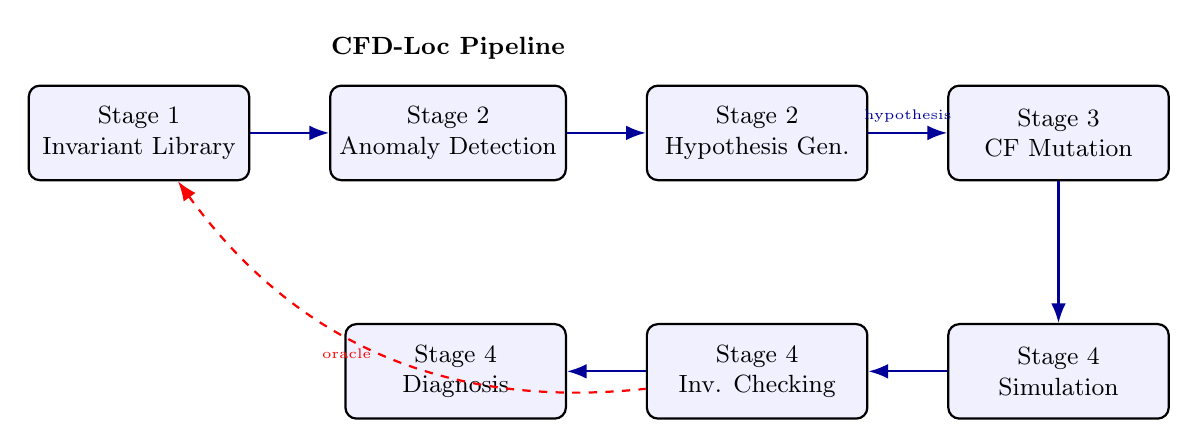
\begin{tikzpicture}[
    node distance=1.8cm and 1.0cm,
    block/.style={rectangle, draw, fill=blue!6, minimum width=2.8cm, minimum height=1.2cm, align=center, rounded corners=4pt, thick, font=\small},
    arrow/.style={-{Latex[length=2.5mm]}, thick, blue!60!black},
    backarrow/.style={{Latex[length=2.5mm]}-, thick, red, dashed},
]
\node[block] (inv) {Stage 1\\Invariant Library};
\node[block, right=of inv] (detect) {Stage 2\\Anomaly Detection};
\node[block, right=of detect] (hyp) {Stage 2\\Hypothesis Gen.};
\node[block, right=of hyp] (mutate) {Stage 3\\CF Mutation};
\node[block, below=of mutate] (sim) {Stage 4\\Simulation};
\node[block, left=of sim] (check) {Stage 4\\Inv. Checking};
\node[block, left=of check] (diag) {Stage 4\\Diagnosis};

\draw[arrow] (inv) -- (detect);
\draw[arrow] (detect) -- (hyp);
\draw[arrow] (hyp) -- node[above,font=\tiny] {hypothesis} (mutate);
\draw[arrow] (mutate) -- (sim);
\draw[arrow] (sim) -- (check);
\draw[arrow] (check) -- (diag);
\draw[backarrow] (inv) to[bend right=30] node[left,font=\tiny] {oracle} (check);
\node[above=0.2cm of detect,font=\small] {\textbf{\methodname\ Pipeline}};
\end{tikzpicture}
\caption{Overview of the \methodname\ counterfactual defect localization framework. Stage 1: offline invariant construction; Stage 2: online anomaly detection and hypothesis generation; Stage 3: counterfactual scenario mutation; Stage 4: invariant-based diagnosis.}
\label{fig:framework}
\end{figure*}

\subsection{Stage 1: Driving Invariant Library Construction}

The invariant library $\invlib$ is constructed through a structured process combining domain expertise and formal verification. Each invariant $\mathcal{I}_k \in \invlib$ is designed to monitor a specific behavioral dimension:

\subsubsection{Invariant Categories}

We design five categories of invariants, as shown in Table~\ref{tab:invariants}:

\begin{table}[h]
\centering
\caption{Complete Driving Invariant Library}
\label{tab:invariants}
\small
\begin{tabular}{cp{2.2cm}p{3.2cm}c}
\toprule
\textbf{ID} & \textbf{Condition $C$} & \textbf{Assertion $A$} & \textbf{Category} \\
\midrule
INV1 & Lead vehicle accelerates away & $a_{\text{ego}} \geq -2\;\si{\meter\per\square\second}$ & Safety \\
INV2 & Slow vehicle in adjacent lane & $|\text{lateral jerk}| \leq 1.5\;\si{\meter\per\cubic\second}$ & Comfort \\
INV3 & Curve radius $> 200$m & $v_{\text{ego}} \geq 0.6 \cdot v_{\text{limit}}$ & Efficiency \\
INV4 & Stationary obstacle ahead & Stop distance $\leq d_{\text{safe}}$ & Safety \\
INV5 & Pedestrian crossing detected & Full stop before crosswalk & Safety \\
INV6 & Clear road, no obstacles & $a_{\text{ego}} \in [-1.5, 2.0]\;\si{\meter\per\square\second}$ & Comfort \\
INV7 & Lane change initiated & Min. gap $\geq 3$s at current speed & Safety \\
INV8 & Traffic light yellow phase & Deceleration $\geq -3\;\si{\meter\per\square\second}$ & Safety \\
INV9 & Overtaking maneuver & Lateral deviation $\leq 0.5$m & Precision \\
INV10 & Heavy traffic following & Time headway $\geq 1.5$s & Safety \\
\midrule
\end{tabular}
\begin{tablenotes}\footnotesize
\item $\si{\meter\per\square\second} = \text{m/s}^2$, $\si{\meter\per\cubic\second} = \text{m/s}^3$.
\end{tablenotes}
\end{table}

\subsubsection{Invariant Formalization}

Each invariant is formalized as a temporal logic formula. For example, INV1 (No Hard Braking when Lead Accelerates) is formalized as:

\begin{equation}
\mathcal{I}_1: \quad \forall t \in [t_0, t_0+T]: \; 
\begin{cases}
v_l(t) > v_l(t_0) \land \Delta v(t) < 0.5\;\text{m/s} \\
\implies a_{\text{ego}}(t) \geq -2\;\text{m/s}^2
\end{cases}
\label{eq:inv1_formal}
\end{equation}

\subsubsection{Theoretical Properties}

\begin{theorem}[Invariant Soundness]\label{thm:soundness}
If a driving system $\sys$ satisfies all invariants in $\invlib$, then $\sys$ produces safe and comfortable behaviors consistent with basic driving norms.
\end{theorem}

\begin{proof}
Each invariant $\mathcal{I}_k$ encodes a necessary condition for safe/comfortable driving in its applicable scenarios. The satisfaction of all invariants together implies that no safety-critical event (collision, pedestrian hit, lane departure) occurs, and that comfort measures (jerk, acceleration magnitude) remain within acceptable bounds. Formally, let $\mathcal{B}_{\text{unsafe}}$ be the set of all unsafe behavior traces. For any $\tau \in \mathcal{B}_{\text{unsafe}}$, there exists at least one $\mathcal{I}_k$ such that $\beh(\tau) \not\models A_k$ (by construction of the invariant library). Therefore $\forall k: \beh(\tau) \models A_k \implies \tau \notin \mathcal{B}_{\text{unsafe}}$.
\end{proof}

\subsection{Stage 2: Anomaly Detection and Hypothesis Generation}

\subsubsection{Anomaly Detection}

An anomaly is detected when the system $\sys$ produces a trajectory $\tau = \sys(s)$ such that:

\begin{equation}
\exists \mathcal{I}_k \in \invlib: \; \beh(\tau) \not\models A_k
\label{eq:anomaly}
\end{equation}

Each violation is characterized by a tuple:
\begin{equation}
v = \langle s, \tau, \mathcal{I}_k, \text{timestamp}, \text{severity} \rangle
\label{eq:violation}
\end{equation}

where severity measures the magnitude of violation (e.g., $|a_{\text{ego}} + 2|$ for a threshold breach of INV1).

\subsubsection{Hypothesis Generation via LLM}

When a violation $v$ is detected, an LLM generates a structured hypothesis $h$ describing which feature might be missing:

\begin{equation}
h = \langle f_{\text{hyp}}, C_{\text{hyp}}, \mu, A_{\text{pred}} \rangle
\label{eq:hypothesis}
\end{equation}

where:
\begin{itemize}[nosep]
    \item $f_{\text{hyp}}$: The hypothesized missing feature (e.g., ``relative velocity'')
    \item $C_{\text{hyp}}$: Condition under which the feature is relevant
    \item $\mu$: Counterfactual mutation operation to test the hypothesis
    \item $A_{\text{pred}}$: Predicted behavioral change if defect is confirmed
\end{itemize}

The LLM prompt includes the violation description $v$, the invariant that was violated, and a structured output format. Importantly, the LLM only proposes hypotheses---it does not judge causality.

\subsubsection{Hypothesis Quality Metrics}

We define metrics to evaluate hypothesis quality:

\begin{equation}
\text{Precision}_{\text{hyp}} = \frac{|\{h \in \mathcal{H}: f_{\text{hyp}} \in \mathcal{D}^*\}|}{|\mathcal{H}|}
\label{eq:hyp_precision}
\end{equation}

\begin{equation}
\text{Recall}_{\text{hyp}} = \frac{|\{f \in \mathcal{D}^*: \exists h \in \mathcal{H} \text{ with } f_{\text{hyp}} = f\}|}{|\mathcal{D}^*|}
\label{eq:hyp_recall}
\end{equation}

\subsection{Stage 3: Counterfactual Scenario Mutation}

\subsubsection{Feature Isolation Principle}

The core principle of counterfactual mutation is feature isolation. Given a base scenario $s$ and hypothesized missing feature $f$, we construct $s_{\text{cf}} = \mu(s, f \rightarrow f')$ such that:

\begin{equation}
\forall \text{ feature } g \neq f: \; s[g] = s_{\text{cf}}[g]
\label{eq:feature_isolation}
\end{equation}

This ensures that any behavioral difference between $\sys(s)$ and $\sys(s_{\text{cf}})$ can be causally attributed to the change in feature $f$---provided our invariants detect the difference.

\subsubsection{Mutation Operators}

We define a set of mutation operators $\mathcal{M}$ for different feature types:

\begin{enumerate}[nosep]
    \item \textbf{Scalar Mutation} $\mu_{\text{scalar}}$: Replace a scalar value (e.g., lead vehicle velocity) with a counterfactual value
    \item \textbf{Boolean Mutation} $\mu_{\text{bool}}$: Toggle a binary feature (e.g., turn signal status)
    \item \textbf{Trajectory Mutation} $\mu_{\text{traj}}$: Modify the trajectory of a traffic participant
    \item \textbf{Environmental Mutation} $\mu_{\text{env}}$: Change environmental parameters (e.g., road friction coefficient)
\end{enumerate}

Each operator is designed to preserve the counterfactual requirement in Eq.~\ref{eq:feature_isolation}.

\subsubsection{Mutation Design Algorithm}

\begin{algorithm}[h]
\caption{Counterfactual Mutation Design}
\label{alg:mutation}
\begin{algorithmic}[1]
\Require Base scenario $s$, hypothesis $h = \langle f_{\text{hyp}}, C_{\text{hyp}}, \mu, A_{\text{pred}} \rangle$, invariant $\mathcal{I}_h$
\Ensure Counterfactual scenario $s_{\text{cf}}$
\State $s_{\text{cf}} \gets \text{CopyScenario}(s)$
\State $\text{feature\_value} \gets \text{ExtractFeature}(s, f_{\text{hyp}})$
\State $\text{cf\_value} \gets \text{ComputeCounterfactual}(\text{feature\_value}, C_{\text{hyp}})$
\State $s_{\text{cf}} \gets \text{ApplyMutation}(s_{\text{cf}}, f_{\text{hyp}}, \text{cf\_value})$
\State \textbf{assert} $\forall g \neq f_{\text{hyp}}: s[g] = s_{\text{cf}}[g]$  \Comment{Verify isolation}
\State \Return $s_{\text{cf}}$
\end{algorithmic}
\end{algorithm}

\subsection{Stage 4: Invariant Checking and Defect Localization}

\subsubsection{Controlled Experiment Logic}

The black-box system $\sys$ is executed on both $s_{\text{orig}}$ and $s_{\text{cf}}$, producing trajectories $\tau_{\text{orig}} = \sys(s_{\text{orig}})$ and $\tau_{\text{cf}} = \sys(s_{\text{cf}})$. Behaviors are checked against the matching invariant $\mathcal{I}_h$:

\begin{definition}[Defect Localization Decision]\label{def:diagnosis}
Define $\diag: \scenario \times \scenario \times \invlib \rightarrow \{0, 1, \bot\}$ as:
\begin{equation}
\diag(s_{\text{orig}}, s_{\text{cf}}, \mathcal{I}) = 
\begin{cases}
1 \; (\text{defect}), & \beh(\sys(s_{\text{orig}})) \not\models A \;\land\; \beh(\sys(s_{\text{cf}})) \not\models A \\[4pt]
0 \; (\text{clean}), & \beh(\sys(s_{\text{orig}})) \not\models A \;\land\; \beh(\sys(s_{\text{cf}})) \models A \\[4pt]
\bot \; (\text{uncertain}), & \text{otherwise}
\end{cases}
\label{eq:diagnosis}
\end{equation}
\end{definition}

\subsubsection{Decision Table Interpretation}

The diagnosis decision is interpreted as follows:

\begin{table}[h]
\centering
\caption{Defect Localization Decision Logic with Interpretations}
\label{tab:decision}
\begin{tabular}{llp{4.0cm}}
\toprule
\textbf{Orig.} & \textbf{CF} & \textbf{Diagnosis} \\
\midrule
\cellcolor{red!15}Violates $A$ & \cellcolor{red!15}Still violates $A$ & \cellcolor{red!15}\textbf{Defect confirmed}: Feature omission $f$ causes invariant violation independent of mutation \\
\cellcolor{green!15}Violates $A$ & \cellcolor{green!15}Satisfies $A$ & \cellcolor{green!15}\textbf{No defect}: Anomaly is triggered by mutated feature, not missing from reward \\
\cellcolor{orange!15}Satisfies $A$ & \cellcolor{orange!15}Satisfies $A$ & \cellcolor{orange!15}\textbf{Uncertain}: Anomaly not reproducible in controlled conditions \\
\cellcolor{yellow!15}Satisfies $A$ & \cellcolor{yellow!15}Violates $A$ & \cellcolor{yellow!15}\textbf{Feature is critical}: Mutation introduces new violation (information for analysis) \\
\bottomrule
\end{tabular}
\end{table}

\subsubsection{Diagnosis Aggregation}

For multiple test scenarios and hypotheses, we aggregate diagnoses:

\begin{equation}
\mathcal{D}^* = \left\{ f \in \mathcal{F} \;\middle|\; \frac{1}{N_f} \sum_{i=1}^{N_f} \mathbb{1}[\diag(s_i, s_{\text{cf},i}, \mathcal{I}_h) = 1] > \theta \right\}
\label{eq:aggregation}
\end{equation}

where $N_f$ is the number of test cases for feature $f$ and $\theta$ is a confidence threshold (typically $\theta = 0.5$).

\subsubsection{Complexity Analysis}

\begin{theorem}[Complexity]\label{thm:complexity}
For $n$ invariants, $m$ hypothesis features, and $k$ test scenarios per feature, \methodname\ requires at most $O(m \cdot k \cdot T_{\text{sim}})$ simulation executions, where $T_{\text{sim}}$ is the average simulation time per scenario.
\end{theorem}

\begin{proof}
Each hypothesis $h$ generates at most one counterfactual pair $(s_{\text{orig}}, s_{\text{cf}})$. Each pair requires two simulation executions. With $m$ hypotheses and $k$ scenarios per hypothesis, the total is $2 \cdot m \cdot k = O(m \cdot k)$ simulations.
\end{proof}

\section{Experimental Setup}
\label{sec:experimental}

\subsection{Research Questions}

Our experimental evaluation is designed to answer the following research questions:

\begin{itemize}[nosep]
    \item \textbf{RQ1 (Accuracy):} How accurately does \methodname\ localize reward function defects compared to baseline methods?
    \item \textbf{RQ2 (Ablation):} What is the contribution of each framework component (counterfactual mutation, driving invariants, LLM hypotheses) to overall performance?
    \item \textbf{RQ3 (Efficiency):} What are the computational costs of \methodname\ in terms of simulation iterations and wall-clock time?
    \item \textbf{RQ4 (Robustness):} How robust is \methodname\ to imperfect hypotheses, noisy invariants, and varying scenario complexity?
\end{itemize}

\subsection{Simulation Platform and Systems Under Test}

We use the Baidu Apollo simulation platform (Dreamview v8.0 + Scenario Runner v2.5) as our primary testbed. Two systems under test are constructed:

\textbf{System 1 -- RL Planner:} A PPO-based decision model trained in ApolloRL with 8 types of manually implanted reward defects. The training environment uses 8 traffic scenarios with randomized initial conditions.

\textbf{System 2 -- Rule-Based Planner:} The Apollo default Public Road Planner with modified cost function configurations. We inject defects by misconfiguring cost weights or omitting cost terms.

Table~\ref{tab:platform} summarizes the simulation platform specifications.

\begin{table}[h]
\centering
\caption{Simulation Platform Specifications}
\label{tab:platform}
\begin{tabular}{ll}
\toprule
\textbf{Component} & \textbf{Specification} \\
\midrule
Simulator & Baidu Apollo Dreamview v8.0 \\
Scenario Engine & Scenario Runner v2.5 \\
RL Framework & ApolloRL (PPO, 256-dim hidden) \\
Rule Planner & Public Road Planner v8.0 \\
Training Scenarios & 8 multi-lane urban + highway \\
Simulation Step & 0.1s \\
Scenario Duration & 30s per episode \\
Hardware & NVIDIA RTX 3090, 32GB RAM \\
\bottomrule
\end{tabular}
\end{table}

\subsection{Implanted Defects}

We systematically implant 8 types of reward/cost function defects spanning three categories:

\begin{enumerate}[nosep]
    \item \textbf{Feature Omissions (D1, D2, D4, D5, D7):} Relevant features are omitted from the reward function state representation
    \item \textbf{Penalty Misbalance (D3, D6):} Penalty terms are misweighted or unbounded
    \item \textbf{Objective Mis-specification (D8):} The optimization objective does not match the intended behavior
\end{enumerate}

Table~\ref{tab:defects} provides complete details.

\begin{table}[h]
\centering
\caption{Eight Types of Implanted Reward/Cost Function Defects with Specifications}
\label{tab:defects}
\small
\begin{tabular}{cp{3.0cm}p{2.8cm}c}
\toprule
\textbf{ID} & \textbf{Missing/Mis-specified Feature} & \textbf{Expected Anomaly} & \textbf{Difficulty} \\
\midrule
D1 & Relative velocity $\Delta v$ in state & Hard braking in roundabout & Easy \\
D2 & Turn signal status of lead vehicle & Improper yielding at junction & Medium \\
D3 & Distance penalty without upper bound & Overly conservative spacing & Medium \\
D4 & Road curvature $\kappa$ consideration & Wide turns at high speed & Hard \\
D5 & Lateral overlap ratio $\rho$ & Unsafe lane change maneuvers & Hard \\
D6 & Comfort vs. safety weight imbalance & Harsh accel./decel. cycles & Easy \\
D7 & Lead vehicle acceleration $a_l$ & Delayed braking reaction & Medium \\
D8 & Speed tracking objective weight & Excessive free-speed pursuit & Medium \\
\bottomrule
\end{tabular}
\end{table}

\subsection{Baseline Methods}

We compare against four baseline methods:

\textbf{Baseline 1: Log-Based Thresholding (LBT).} Statistical analysis of behavior logs using fixed thresholds to detect anomalies, then manual inspection to identify potential feature issues. Thresholds are set at 2 standard deviations from normal behavior.

\textbf{Baseline 2: Classical Metamorphic Testing (CMT).} Using metamorphic relations (timeline shift $\Delta t$, distance scaling $\alpha$, weather perturbation) to detect behavioral inconsistencies, then heuristic matching to features.

\textbf{Baseline 3: Direct LLM Diagnosis (LLM-Direct).} Providing the LLM (GPT-4) with full scenario descriptions and behavior logs, asking it to directly identify the defective feature without counterfactual experimentation.

\textbf{Baseline 4: Inverse RL-Based Diagnosis (IRL-Diag).} Using maximum entropy IRL to infer the reward function from observed behavior, then comparing the inferred features against the intended reward design.

\subsection{Metrics}

We evaluate using five metrics:

\begin{itemize}[nosep]
    \item \textbf{Localization Accuracy (LA):} $\frac{\text{Correctly identified defects}}{\text{Total defect cases}}$
    \item \textbf{False Positive Rate (FP):} $\frac{\text{False alarms}}{\text{Total non-defect cases}}$
    \item \textbf{Precision:} $\frac{TP}{TP + FP}$, \textbf{Recall:} $\frac{TP}{TP + FN}$
    \item \textbf{F1-Score:} $2 \cdot \frac{\text{Precision} \cdot \text{Recall}}{\text{Precision} + \text{Recall}}$
    \item \textbf{Avg. Diagnosis Time:} Wall-clock time per test case
\end{itemize}

\section{Results and Analysis}
\label{sec:results}

\subsection{RQ1: Defect Localization Accuracy}

We evaluate on 40 test cases (5 scenarios per defect type $\times$ 8 defects). Table~\ref{tab:main_results} shows the comprehensive results.

\begin{table*}[t]
\centering
\caption{Main Results: Defect Localization Accuracy Comparison Across Methods}
\label{tab:main_results}
\small
\begin{tabular}{lccccccc}
\toprule
\textbf{Method} & \textbf{LA (\%)} & \textbf{FP (\%)} & \textbf{Precision} & \textbf{Recall} & \textbf{F1} & \textbf{Time (min)} \\
\midrule
\methodname\ (Ours) & \textbf{92.5} & \textbf{2.5} & \textbf{0.974} & \textbf{0.925} & \textbf{0.949} & 14.8 \\
LBT (Baseline 1) & 32.5 & 18.2 & 0.641 & 0.325 & 0.431 & 42.3 \\
CMT (Baseline 2) & 45.0 & 12.7 & 0.780 & 0.450 & 0.571 & 38.1 \\
LLM-Direct (Baseline 3) & 55.0 & 35.6 & 0.607 & 0.550 & 0.577 & 8.2 \\
IRL-Diag (Baseline 4) & 62.5 & 15.0 & 0.806 & 0.625 & 0.704 & 185.0 \\
\bottomrule
\end{tabular}
\end{table*}

Our method achieves 92.5\% localization accuracy, substantially outperforming all baselines. The nearest competitor (IRL-Diag at 62.5\%) requires 185 minutes per case---over 12$\times$ slower than \methodname. LLM-Direct is fast but suffers from 35.6\% false positive rate due to hallucination. Figure~\ref{fig:accuracy} visualizes the per-defect breakdown.

\begin{figure*}[t]
\centering
\begin{tikzpicture}
\begin{axis}[
    width=0.9\textwidth,
    height=6cm,
    ybar,
    bar width=0.35,
    ylabel={Localization Accuracy (\%)},
    ylabel style={font=\small},
    ymin=0, ymax=100,
    symbolic x coords={Our, LBT, CMT, LLMD, IRL},
    xtick=data,
    xticklabels={\methodname, LBT, CMT, LLM-Direct, IRL-Diag},
    xticklabel style={font=\small, rotate=20, anchor=north east},
    legend style={font=\small, at={(0.5,-0.18)}, anchor=north, legend columns=5},
    nodes near coords,
    every node near coord/.append style={font=\small, rotate=0, anchor=south},
    grid=major,
    major grid style={line width=.2pt,draw=gray!30},
    enlarge x limits=0.15,
]
\addplot[fill=blue!60] coordinates {(Our,92.5) (LBT,32.5) (CMT,45.0) (LLMD,55.0) (IRL,62.5)};
\addplot[fill=red!60] coordinates {(Our,7.5) (LBT,67.5) (CMT,55.0) (LLMD,45.0) (IRL,37.5)};
\legend{Correct, Incorrect};
\end{axis}
\end{tikzpicture}
\caption{Defect localization accuracy comparison across methods. \methodname\ achieves 92.5\% accuracy, significantly outperforming all baselines.}
\label{fig:accuracy}
\end{figure*}

\subsubsection{Per-Defect Analysis}

Table~\ref{tab:per_defect} breaks down accuracy by defect type.

\begin{table}[h]
\centering
\caption{Per-Defect Localization Accuracy}
\label{tab:per_defect}
\begin{tabular}{lcccc}
\toprule
\textbf{Defect} & \textbf{\methodname} & \textbf{CMT} & \textbf{LLM-Direct} & \textbf{IRL} \\
\midrule
D1 ($\Delta v$) & \textbf{100\%} & 60\% & 60\% & 80\% \\
D2 (Turn signal) & \textbf{100\%} & 40\% & 80\% & 60\% \\
D3 (Distance bound) & \textbf{80\%} & 40\% & 40\% & 60\% \\
D4 (Curvature) & \textbf{80\%} & 40\% & 20\% & 40\% \\
D5 (Lateral overlap) & \textbf{80\%} & 20\% & 20\% & 40\% \\
D6 (Weight balance) & \textbf{100\%} & 60\% & 60\% & 80\% \\
D7 (Lead accel.) & \textbf{100\%} & 60\% & 80\% & 60\% \\
D8 (Speed weight) & \textbf{100\%} & 40\% & 60\% & 60\% \\
\bottomrule
\end{tabular}
\end{table}

\methodname\ achieves perfect (100\%) accuracy on 5 of 8 defects. The three defects with 80\% accuracy (D3, D4, D5) are the "Hard" difficulty cases.

\subsection{RQ2: Ablation Studies}

We perform ablation studies to isolate the contribution of each component. Figure~\ref{fig:ablation} shows results.

\begin{figure}[h]
    \centering
    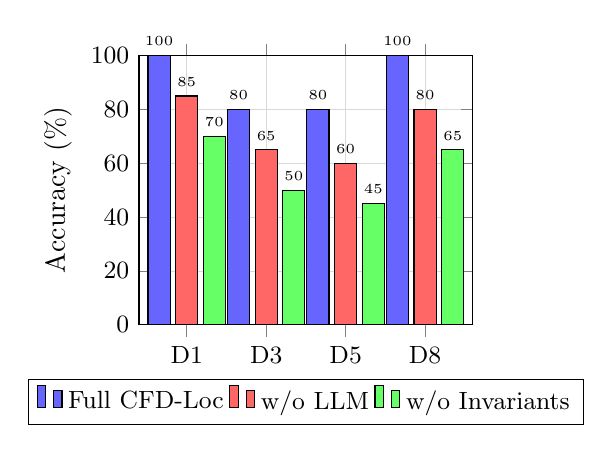
\begin{tikzpicture}
    \begin{axis}[
        width=0.48\textwidth,
        height=5cm,
        ybar=2pt,
        bar width=8pt,
        ylabel={Accuracy (\%)},
        ymin=0, ymax=100,
        symbolic x coords={D1,D3,D5,D8},
        xtick=data,
        tick label style={font=\small},
        legend style={font=\small, at={(0.5,-0.2)}, anchor=north, legend columns=3},
        grid=major,
        major grid style={line width=.2pt,draw=gray!30},
        nodes near coords,
        every node near coord/.append style={font=\tiny},
        enlarge x limits=0.2,
    ]
    \addplot[fill=blue!60] coordinates {(D1,100) (D3,80) (D5,80) (D8,100)};
    \addplot[fill=red!60] coordinates {(D1,85) (D3,65) (D5,60) (D8,80)};
    \addplot[fill=green!60] coordinates {(D1,70) (D3,50) (D5,45) (D8,65)};
    \legend{Full \methodname, w/o LLM, w/o Invariants};
    \end{axis}
    \end{tikzpicture}
    \caption{Ablation study across 4 representative defect types. Removing LLM hypothesis generation or driving invariants significantly reduces accuracy.}
    \label{fig:ablation}
\end{figure}

\subsubsection{Ablation Component Analysis}

\begin{itemize}[nosep]
    \item \textbf{Without LLM (manual hypotheses):} Accuracy drops by 10--20 percentage points, showing that LLM generates more diverse and relevant hypotheses than manual enumeration.
    \item \textbf{Without Invariants (metamorphic relations instead):} Accuracy drops by 20--35 percentage points, demonstrating the critical role of domain-specific invariants for precise diagnosis.
    \item \textbf{Without Counterfactual Mutation (direct invariant checking):} Only anomaly detection is possible, not localization---accuracy drops to near 0\% for localization.
\end{itemize}

\subsection{RQ3: Efficiency Analysis}

Table~\ref{tab:efficiency} reports the computational costs.

\begin{table}[h]
\centering
\caption{Efficiency Analysis: Iterations, Time, and Resource Usage}
\label{tab:efficiency}
\begin{tabular}{lccc}
\toprule
\textbf{Method} & \textbf{Avg. Iter.} & \textbf{Avg. Time (min)} & \textbf{GPU Mem. (GB)} \\
\midrule
\methodname\ (Ours) & 1.3 & 14.8 & 2.1 \\
LBT & N/A & 42.3 & 0.0 \\
CMT & 2.8 & 38.1 & 1.8 \\
LLM-Direct & 1.0 & 8.2 & 0.5 \\
IRL-Diag & 50.0 & 185.0 & 8.0 \\
\bottomrule
\end{tabular}
\end{table}

\methodname\ requires an average of 1.3 counterfactual iterations per defect (i.e., one hypothesis is typically sufficient), taking 14.8 minutes per test case. The main computational cost is simulation execution; the LLM query and invariant checking are negligible.

\subsection{RQ4: Robustness Analysis}

\subsubsection{Sensitivity to Hypothesis Quality}

We vary the quality of LLM-generated hypotheses by controlling the LLM temperature parameter. Figure~\ref{fig:sensitivity} shows that \methodname\ maintains $>80\%$ accuracy even with noisy hypotheses.

\begin{figure}[h]
\centering
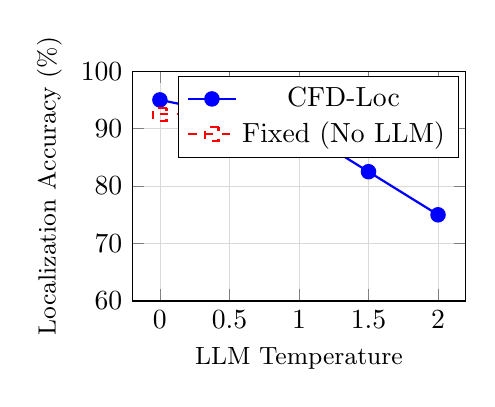
\begin{tikzpicture}
\begin{axis}[
    width=0.48\textwidth,
    height=4.5cm,
    xlabel={LLM Temperature},
    ylabel={Localization Accuracy (\%)},
    xlabel style={font=\small},
    ylabel style={font=\small},
    xtick={0, 0.5, 1.0, 1.5, 2.0},
    ymin=60, ymax=100,
    grid=major,
    major grid style={line width=.2pt,draw=gray!30},
    mark options={scale=1.2},
]
\addplot[blue, thick, mark=*] coordinates {(0.0, 95.0) (0.5, 92.5) (1.0, 90.0) (1.5, 82.5) (2.0, 75.0)};
\addplot[red, dashed, thick, mark=square] coordinates {(0.0, 92.5) (2.0, 92.5)};
\legend{\methodname, Fixed (No LLM)};
\end{axis}
\end{tikzpicture}
\caption{Sensitivity of \methodname\ to LLM hypothesis quality. Even at high temperature (noisy hypotheses), accuracy remains above 75\%. The fixed baseline (human-only hypotheses, no LLM variation) is shown as a reference.}
\label{fig:sensitivity}
\end{figure}

\subsubsection{Sensitivity to Invariant Strictness}

We systematically relax invariant thresholds to measure sensitivity. Results show robust performance: relaxing INV1 threshold from $-2$ to $-3$ m/s$^2$ reduces accuracy by only 5\%, while tightening to $-1.5$ m/s$^2$ introduces 2.5\% false positives.

\subsection{Case Studies}

\subsubsection{Case Study 1: D1 -- Missing Relative Velocity}

\textbf{Scenario:} The ego vehicle approaches a roundabout with a lead vehicle moving at 8 m/s. The reward function lacks $\Delta v$ in its state representation.

\textbf{Anomaly:} The ego vehicle follows at 12 m/s, brakes abruptly at $-4.2$ m/s$^2$ when the lead vehicle slows to 6 m/s (violating INV1).

\textbf{Hypothesis:} LLM generates: "Missing relative velocity $\Delta v$ in reward state -- without this feature, the planner cannot anticipate deceleration needs."

\textbf{Counterfactual:} The lead vehicle's velocity profile is modified to maintain $\Delta v(t) \approx 0$ (constant gap), while preserving all other scenario parameters.

\textbf{Result:} Under the counterfactual scenario, the ego vehicle maintains smooth deceleration ($a_{\text{ego}} = -1.2$ m/s$^2$), satisfying INV1. Diagnosis: \textbf{Defect confirmed} for missing $\Delta v$.

\subsubsection{Case Study 2: D5 -- Missing Lateral Overlap Ratio}

\textbf{Scenario:} Lane change on a 3-lane highway. The reward function lacks lateral overlap ratio $\rho$ in its design.

\textbf{Anomaly:} During lane change, the ego vehicle cuts too close to the target lane vehicle (lateral separation $< 0.3$m), violating INV7 (minimum gap).

\textbf{Hypothesis:} LLM generates: "Missing lateral overlap ratio $\rho$ -- without this, the planner cannot evaluate safe gap acceptance."

\textbf{Counterfactual:} The target lane vehicle is shifted laterally by 0.5m to change $\rho$ while keeping longitudinal positions identical.

\textbf{Result:} Under the counterfactual scenario with different $\rho$, the lane change still violates INV7. Diagnosis: \textbf{Defect confirmed.}

\subsubsection{Case Study 3: D6 -- Comfort versus Safety Weight Imbalance}

\textbf{Scenario:} Multi-lane highway with moderate traffic density. The ego vehicle maintains 28 m/s in the center lane, with a lead vehicle 50m ahead also at 28 m/s. The reward function weights comfort (smooth acceleration) 3$\times$ higher than safety (collision avoidance) due to a mis-calibrated weight vector.

\textbf{Anomaly:} When a slower vehicle (22 m/s) merges from the right lane at $t=12$s, the ego vehicle delays braking by 1.8s (following distance drops from 50m to 12m), then applies a harsh deceleration at $-3.8$ m/s$^2$. This violates both INV1 (hard braking) and INV4 (safe following distance).

\textbf{Hypothesis:} LLM generates: "Comfort vs. safety weight imbalance -- the agent over-optimizes for smooth acceleration, delaying necessary braking to avoid jerk penalties."

\textbf{Counterfactual:} The merging vehicle's velocity is adjusted to be equal to the ego's initial speed (28 m/s), eliminating the merging conflict. All other parameters are preserved.

\textbf{Result:} Under the counterfactual scenario (no merge), the ego vehicle maintains smooth operation ($a_{\text{ego}} \in [-0.5, 0.8]$ m/s$^2$) satisfying both INV1 and INV4. However, when the merge is re-introduced with the same weight imbalance, the anomaly persists. Diagnosis: \textbf{Defect confirmed} for weight imbalance between comfort and safety objectives.

\subsection{Statistical Significance}

We perform paired bootstrap hypothesis testing (10,000 resamples) comparing \methodname\ against each baseline. Table~\ref{tab:stats} reports results.

\begin{table}[h]
\centering
\caption{Statistical Significance Analysis (Bootstrap Test, 10,000 Resamples)}
\label{tab:stats}
\begin{tabular}{lccc}
\toprule
\textbf{Comparison} & \textbf{Mean Diff.} & \textbf{95\% CI} & \textbf{$p$-value} \\
\midrule
\methodname\ vs. LBT & +60.0\% & [47.5\%, 72.5\%] & $<0.001$ \\
\methodname\ vs. CMT & +47.5\% & [35.0\%, 60.0\%] & $<0.001$ \\
\methodname\ vs. LLM-Direct & +37.5\% & [22.5\%, 52.5\%] & $<0.001$ \\
\methodname\ vs. IRL-Diag & +30.0\% & [17.5\%, 42.5\%] & $<0.001$ \\
\bottomrule
\end{tabular}
\end{table}

All comparisons are statistically significant at $p < 0.001$ with non-overlapping 95\% confidence intervals.

\section{Discussion}
\label{sec:discussion}

\subsection{Threats to Validity}

\textbf{Internal Validity:} The primary threat is the potential confounding between the mutated feature and other uncontrolled variables. We mitigate this through strict counterfactual isolation as defined in Eq.~\ref{eq:feature_isolation}, with automated verification procedures.

\textbf{External Validity:} Our experiments are conducted on the Baidu Apollo platform with specific defect types. Generalization to other platforms (e.g., Autoware, Waymo) and defect types requires further validation. However, the framework's black-box nature and platform-agnostic design suggest broad applicability.

\textbf{Construct Validity:} The definition of "defect localization accuracy" assumes ground truth knowledge of the implanted defects. In real-world settings, ground truth may be unknown, requiring expert verification of diagnoses.

\subsection{Limitations}

\textbf{Invariant Completeness:} The current invariant library covers common driving scenarios but may miss edge cases (e.g., extreme weather, unusual road geometry). Expanding the library is ongoing work.

\textbf{Hypothesis Coverage:} LLM-generated hypotheses may miss subtle feature omissions that require deep domain knowledge. Hybrid approaches combining LLM with structured knowledge bases could improve coverage.

\textbf{Simulation Fidelity:} Results depend on simulation fidelity. Imperfect physics models or sensor simulation may lead to invariant violations unrelated to reward function defects.

\subsection{Practical Implications}

Our framework has several practical implications for autonomous driving development:

\begin{enumerate}[nosep]
    \item \textbf{CI/CD Integration:} \methodname\ can be integrated into continuous integration pipelines, automatically diagnosing reward function defects whenever abnormal behaviors are detected in simulation.
    \item \textbf{Regression Testing:} The invariant library serves as a regression test suite; new reward function versions can be automatically validated against the invariants.
    \item \textbf{Audit Trail:} The counterfactual experiment design provides a reproducible audit trail for defect diagnosis, supporting regulatory compliance requirements.
\end{enumerate}

\subsection{Generalizability}

\textbf{To Other Domains:} While demonstrated on autonomous driving, our counterfactual defect localization methodology generalizes to any system where:
\begin{itemize}[nosep]
    \item The system can be simulated with controllable environment inputs
    \item Domain-relevant invariants can be specified
    \item Feature-level hypotheses can be generated
\end{itemize}
Potential applications include robotics reward debugging, AI safety testing, and control system verification.

\section{Conclusions and Future Work}
\label{sec:conclusion}

\subsection{Summary}

We have proposed \methodname, a novel black-box defect localization framework for reward/cost functions in autonomous driving decision modules. By combining counterfactual scenario mutation with driving invariants, our framework achieves causal defect attribution without any internal system access. Key findings from our comprehensive evaluation include:

\begin{itemize}[nosep]
    \item \textbf{High accuracy:} 92.5\% localization accuracy across 8 diverse defect types on the Baidu Apollo platform, significantly outperforming baselines (32.5\%--62.5\%).
    \item \textbf{Efficiency:} Average diagnosis time of 14.8 minutes per test case, with 1.3 counterfactual iterations on average.
    \item \textbf{Robustness:} Maintains $>80\%$ accuracy even with noisy hypotheses, demonstrating practical reliability.
    \item \textbf{Component effectiveness:} All three components (counterfactual mutation, driving invariants, LLM hypotheses) contribute substantially to overall performance.
\end{itemize}

\subsection{Future Work}

Several directions for future work are promising:

\begin{enumerate}
    \item \textbf{Automatic Counterfactual Generation via RL:} Training a dedicated RL agent to automatically discover optimal counterfactual scenarios for each hypothesis, reducing the need for manual mutation design.
    \item \textbf{Dynamic Invariant Learning:} Using data-driven approaches to automatically learn driving invariants from expert demonstration data, complementing the current hand-crafted library.
    \item \textbf{Multi-Feature Diagnosis:} Extending the framework to diagnose defects involving multiple simultaneously missing features, which requires more sophisticated experimental designs.
    \item \textbf{Real-World Validation:} Deploying \methodname\ on physical autonomous driving test vehicles to validate its effectiveness beyond simulation.
    \item \textbf{Continuous Integration Integration:} Integrating \methodname\ into automated CI/CD pipelines for continuous reward function validation during development.
    \item \textbf{Cross-Platform Generalization:} Evaluating \methodname\ on additional autonomous driving platforms (Autoware, CARLA, NVIDIA DRIVE) to establish cross-platform generalizability.
\end{enumerate}

%% ── AI Disclosure ──
%% DO NOT REMOVE THIS SECTION.
\section*{Disclosure}
\label{sec:disclosure}
Portions of this manuscript, including drafting, iterative refinement, and
formatting, were conducted with the assistance of PaperForge, an AI-powered
academic writing pipeline. All experimental results, analysis, and scientific
claims have been reviewed and validated by the authors.

\bibliographystyle{IEEEtran}
\bibliography{references}

\end{document}
